\documentclass[10pt,twocolumn,letterpaper]{article}

\usepackage{cvpr}
\usepackage{times}
\usepackage{epsfig}
\usepackage{graphicx}
\usepackage{amsmath}
\usepackage{amssymb}
\usepackage[english]{babel}
\usepackage{blindtext}
\usepackage{multirow}

% Include other packages here, before hyperref.

% If you comment hyperref and then uncomment it, you should delete
% egpaper.aux before re-running latex.  (Or just hit 'q' on the first latex
% run, let it finish, and you should be clear).
\usepackage[breaklinks=true,bookmarks=false]{hyperref}

\cvprfinalcopy % *** Uncomment this line for the final submission

\def\cvprPaperID{****} % *** Enter the CVPR Paper ID here
\def\httilde{\mbox{\tt\raisebox{-.5ex}{\symbol{126}}}}

% Pages are numbered in submission mode, and unnumbered in camera-ready
%\ifcvprfinal\pagestyle{empty}\fi
\setcounter{page}{4321}
\begin{document}

%%%%%%%%% TITLE
\title{SignNet: Recognize Alphabets in the American Sign Language in Real Time}

\author{
Zeqiang Lai\\
Beijing Institute of Technology\\
{\tt\small laizeqiang@outlook.com}
% For a paper whose authors are all at the same institution,
% omit the following lines up until the closing ``}''.
% Additional authors and addresses can be added with ``\and'',
% just like the second author.
% To save space, use either the email address or home page, not both
\and
Zhiyuan Liang\\
Beijing Institute of Technology\\
{\tt\small secondauthor@i2.org}
\and
Kexiang Huang\\
Beijing Institute of Technology\\
{\tt\small thirdauthor@i2.org}
}

\maketitle
%\thispagestyle{empty}

%%%%%%%%% ABSTRACT
\begin{abstract}
   The ABSTRACT is to be in fully-justified italicized text, at the top
   of the left-hand column, below the author and affiliation
   information. Use the word ``Abstract'' as the title, in 12-point
   Times, boldface type, centered relative to the column, initially
   capitalized. The abstract is to be in 10-point, single-spaced type.
   Leave two blank lines after the Abstract, then begin the main text.
   Look at previous CVPR abstracts to get a feel for style and length.
   The code has been made available at \url{https://github.com/Zeqiang-Lai/SignNet}
\end{abstract}

%%%%%%%%% BODY TEXT
\section{Introduction}

\blindtext

\begin{figure}[t]
\begin{center}
 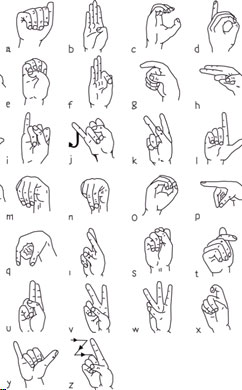
\includegraphics[width=0.8\linewidth]{imgs/NIDCD-ASL-hands-2014.jpg}
\end{center}
\caption{Sign Language Reference}
\label{fig:long}
\end{figure}


\blindtext

%%%%%%%%% Related Work


\section{Related Work}

\begin{figure*}[ht]
\begin{center}
\fbox{\rule{0pt}{2in} \rule{.9\linewidth}{0pt}}
\end{center}
   \caption{Network architecture}
\label{fig:arch}
\end{figure*}

\blindtext

\blindtext

%%%%%%%%% Model Description

\section{SignNet}

As it is mentioned before, we formulate sign language recognition task as a classification problem and we use a modified version of VGG Network \cite{simonyan2014very} to train a classifier for images with different signs. 

In detail, our modifications can be summaried as followed(See Figure \ref{fig:arch}). First, we reduce the size of last fully connected network from 4096 to 512. Secondly, we reduce the number of filter of the intermediate convolutional blocks. We make these modifications based on the requirement of live recognition and the assumption that VGG is way to large for the sign language recognition task, which was shown to be correct by the experiment on the ASL Dataset.

The exact network architecture can be described in table\ref{table:arch}. The total number of parameter is 10m approximately and the model can achieve 20+fps on an Intel Core I7 CPU.  

\begin{table}[h]
\begin{center}
\begin{tabular}{|l|c|c|c|c|}
\hline
Layer Type & Kernel & Stride & Outputs & Acivation \\
\hline\hline
Conv & 1$\times$3 & 1 & 1$\times$31$\times$3 & ReLU\\
Conv & 1$\times$3 & 1 & 1$\times$31$\times$3 & ReLU\\
Conv & 1$\times$3 & 1 & 1$\times$31$\times$3 & ReLU\\
Conv & 1$\times$3 & 1 & 1$\times$31$\times$3 & ReLU\\
Conv & 1$\times$3 & 1 & 1$\times$31$\times$3 & ReLU\\
FC & 1$\times$3 & 1 & 1$\times$31$\times$3 & ReLU\\
\hline
\end{tabular}
\end{center}
\caption{Results.  Ours is better.}
\label{table:arch}
\end{table}


%%%%%%%%% Experiments

\section{Vanilla Experiments}

[Need edit] In this section, we introduce the experiments we have conducted using the model described in the previous section.

\subsection{ASL Dataset}

ASL Alphabet\cite{noauthor_asl_nodate} is a collection of images of alphabets from the American Sign Language, which is public available on Kaggle. The training data set contains 87,000 images which are 200$\times$200 pixels. There are 29 classes, of which 26 are for the letters A-Z and 3 classes for SPACE, DELETE and NOTHING. The test data set contains a mere 29 images, which is too small for an effective test.

For testing, we use another dataset - ASL Alphabet Test\cite{noauthor_asl_nodate-1}. This dataset is collected by a different person and it consists of 870 images with various background. There are 30 images for each symbol, A-Z, delete, space, and nothing and every image is 200$\times$200 8-bit photo, which is the same as it is in ASL Alphabet. 

See Figure \ref{fig:asl} for a preview of ASL Alphabet and ASL Alphabet Test.

\begin{figure}[h]
\begin{center}
\fbox{\rule{0pt}{2in} \rule{0.9\linewidth}{0pt}}
   %\includegraphics[width=0.8\linewidth]{egfigure.eps}
\end{center}
 \caption{Preivew of ASL Alphabet and ASL Alphabet Test}
\label{fig:asl}
\end{figure}


\subsection{Training Detail}\label{sec:training_detail}

We implement our model with Pytorch, and train it with cross entropy loss and Adam optimizer\cite{kingma2014adam} with default parameters. The learning rate is set to 0.0001 for the first epoch, and decayed by a ratio of 0.7 every other epoch. 

During training, we randomly flip images horizontally. After that, the images are converted into grayscale and resized to 64$\times$64 to reduce computational complexity. 

\subsection{Results}

The training and testing result is shown in table\ref{table:result}. We can see   that the model can overfit on the training set, but it works badly on test set. This poor performance might be the result of the lack of background variation in the training set, or the regularization on the model. In any cases, current model work 

\begin{table}[h]
\begin{center}
\begin{tabular}{|l|c|}
\hline
Dataset & Accuracy \\
\hline\hline
ASL Alphabet(Training) & Frumpy \\
ASL Alphabet Test & Frobbly \\
Our ASL Test Set & Makes one's heart Frob\\
\hline
\end{tabular}
\end{center}
\caption{Results.   Ours is better.}
\label{table:result}
\end{table}

\section{Improvement}

The ASL Alphabet dataset has small background variations and it is hard to train a model that works well in real environment, which is shown in the experiments mentioned in the previous section.

As a result, we decided to make a dataset on our own. In order to reduce the negative effect of background on prediction, we use background subtraction technique to remove it while recording dataset, and we use the same method to remove background in testing and inference stages. In this way, we can basically obtain a model that is able to work under limited environment.

\subsection{Custom Dataset}

Instead of collecting more data with different backgrounds, we choose to make a dataset without background directly, because the former is generally time-consuming and laborious.

Similar to the ASL Alphabet, our custom dataset also consists 29 types of gestures where each type includes 900 and 300 images (200px$\times$200px) for training and testing, respectively. Background of each video is removed using a background subtraction algorithm, as it is shown in Figure \ref{fig:dataset}.

\begin{figure}[h]
\begin{center}
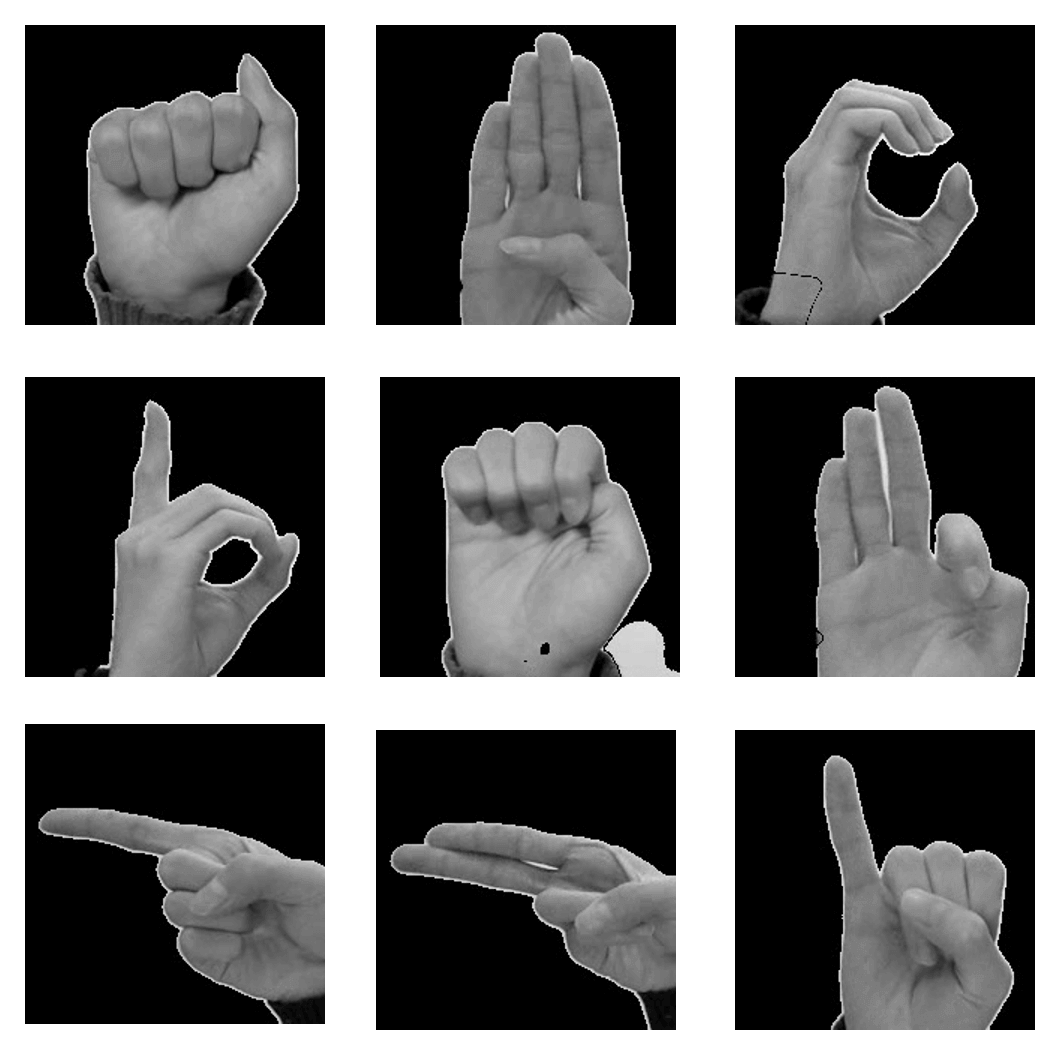
\includegraphics[width=0.8\linewidth]{imgs/dataset.png}
\end{center}
   \caption{Origin, mask and grayscale hand images}
\label{fig:dataset}
\end{figure}


\subsection{Background Subtraction}

We choose Running Average Background Subtraction algorithm to detect and remove background, because it is fast and easy to implement.

The key idea of this algorithm is to compute a reference background image using running average of first few frames in a video, and subtract the current image with respect to the reference background, and finally compare it with  to the certain threshold. Pixels that exceed threshold are considered to be foreground, while all the others are background.
 
 After comparison, we could get a background mask. Instead of using binary mask directly, we use the mask to remove background to get a grayscale hand image, because some signs require counting fingers to be recognized correctly. See Figure \ref{fig:dataset}.


\subsection{Experiment}

\paragraph{Training Setting}
With the new custom dataset, we use the same loss, optimizer, and data preprocessing techniques to train a new recognition model. (See previous section \ref{sec:training_detail} for more training detail).

\paragraph{Quantitative Results}
It takes about 5 epochs for the recognition model to converge and another 15 epochs for further tuning. As it is shown in Table \ref{table:result}, our model works perfectly on training set, but the test accuracy is slightly lower.

\begin{table}[h]
\begin{center}
\begin{tabular}{|l|c|}
\hline
Dataset & Accuracy \\
\hline\hline
Custom Train & 25804/25809 (100\%) \\
Custom Test & 7364/8700 (85\%) \\
\hline
\end{tabular}
\end{center}
\caption{Results on custom datasets}
\label{table:result}
\end{table}

\paragraph{Error Analysis} Figure \ref{fig:confusion} shows the confusion matrix on the custom test set. We can observe from the figure that the majority of gestures can be recognized correctly, but there are some gestures are frequently misclassified to certain types. For example, almost all the gesture M are misclassified to N. If we have a look on the gestures of M and N (See Figure), it can be understood that our model work bad on these two ones, because they are similar to each other. In summary, our model work well on the most part of cases, but can be confused with some similar gestures, which might be improved with more training examples.


\begin{figure}[h]
\begin{center}
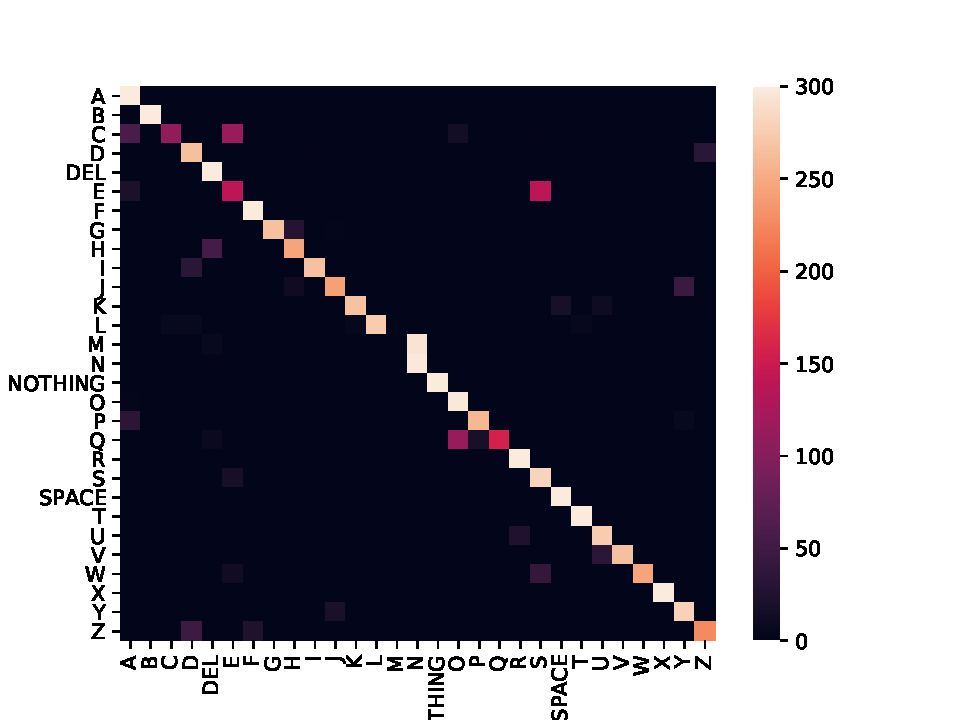
\includegraphics[width=1\linewidth]{imgs/confusion}
\end{center}
   \caption{Confusion matrix on custom test set}
\label{fig:confusion}
\end{figure}

\paragraph{Speed Test}
To evaluate the run-time performance of our approach, we perform a set of tests under different hardwares and platforms. As it is shown in Table \ref{table:fps}, our model can easily achieve real time performance both GPU and CPU where tests are conducted on a series of static images (rows of type static). To demonstrate the performance on live stream, we also implement a live script using OpenCV. The test result with such script achieve 400fps on GPU and is approximately real-time on CPU.  

\begin{table}[h]
\begin{center}
\begin{tabular}{|l|l|l|l|}
\hline
Hardware              & Platform                & Type   & FPS \\ \hline\hline
\multirow{2}{*}{Intel Core i7}   & \multirow{2}{*}{macOS 10.15.7}  & live   & 15.73  \\ \cline{3-4} 
                      &                         & static & 81.00  \\ \hline
\multirow{2}{*}{Nvidia RTX 2080} & \multirow{2}{*}{Windows} & live   & 90  \\ \cline{3-4} 
                      &                         & static & 400 \\ \hline
Nvidia GTX 1070 & Ubuntu 20.04.1 & static & 453.78 \\ \hline                    
\end{tabular}
\end{center}
\caption{Average FPS of our model in different settings. Type "live" means it is tested using our live\_demo script which uses OpenCV to record video in real time, and type "static" means it is tested using static images.}
\label{table:fps}
\end{table}

%%%%%%%%% Conclusion

\section{Conclusion}
\blindtext



{\small
\bibliographystyle{ieee_fullname}
\bibliography{egbib}
}

\end{document}
